%!TEX root = paper.tex
\begin{figure}[h]
  \centering
  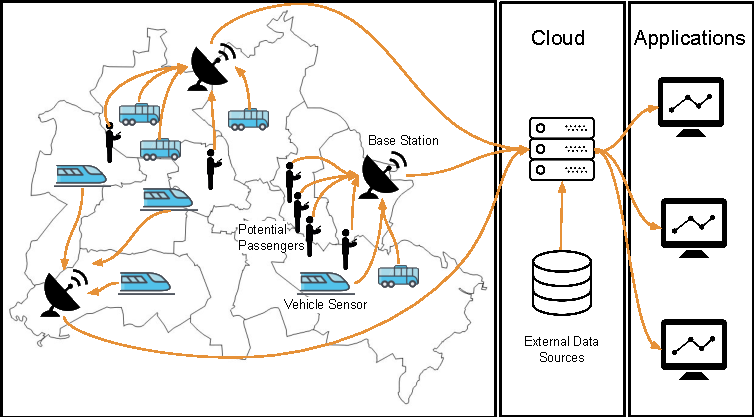
\includegraphics[width=\linewidth]{figs/iot_scenario}
  \caption{Common IoT Infrastructure.}
  \label{fig:iot-app-scenario}
\end{figure}
\section{Background}
\label{sec:background}
% 
% In this section, we discuss present our demonstrated IoT use case and point out why state of the art cloud-based SPEs fall short to address those.
% 
% \subsection{Public Transport as an IoT Scenario}

In this section, we address the basic concepts needed to understand Nalisnick and Smyth's \textit{Stick-Breaking Variational Autoencoders}~\cite{nalisnick2016stickbreaking}. Therefore, we cover the general concepts of \textit{Autoencoders} \textcolor{red}{insert reference}, moving on to \textit{Variational Autoencoders} \textcolor{red}{insert reference}, diving into \textit{Stochastic Gradient Variational Bayes} \textcolor{red}{insert reference}, and finishing with \textit{Stick-Breaking Processes} \textcolor{red}{insert reference}.

\subsection{Autoencoders}

\textcolor{red}{autoencoders learn a “compressed representation” of input (could be image,text sequence etc.) automatically by first compressing the input (encoder) and decompressing it back (decoder) to match the original input. The learning is aided by using distance function that quantifies the information loss that occurs from the lossy compression. So learning in an autoencoder is a form of unsupervised learning (or self-supervised as some refer to it) - there is no labeled data.}


\subsection{Variational Autoencoders}

\textcolor{red}{Instead of just learning a function representing the data ( a compressed representation) like autoencoders, variational autoencoders learn the parameters of a probability distribution representing the data. Since it learns to model the data, we can sample from the distribution and generate new input data samples. So it is a generative model like, for instance, GANs.}

\subsection{Stochastic Gradient Variational Bayes}

\subsection{Stick-Breaking Processes}